\subsection{AHTR Temperature Model with Moltres}
\begin{frame}
    \frametitle{AHTR Temperature Model}
    \visible<1->{An \textbf{AHTR temperature model} captures \textbf{thermal feedback 
    effects}, absent from the purely neutronics FHR Benchmark simulations.} 

    \visible<2->{\begin{block}{Moltres \cite{lindsay_introduction_2018}}
        \begin{itemize}
			\item An application built on the \gls{MOOSE} framework, for the simulation of 
            MSRs
            \item \gls{MOOSE} \cite{gaston_moose:_2009} is an open source finite
			element framework written in \texttt{C++} that
			relies on Libmesh and PETSc for meshing and PDE solving capabilities
			\item Moltres can run transient, implicitly coupled
			neutronics/thermal-hydraulics simulations
			\begin{itemize}
				\item Multi-group neutron diffusion (arbitrary no. of groups)
				\item Delayed neutron precursor decay (with advection)
				\item Incompressible Navier-Stokes for temperature
				advection-diffusion
			\end{itemize}
		\end{itemize}
    \vspace{-0.2cm}
    \end{block}}
    \visible<3->{\begin{block}{AHTR Temperature Model with Moltres}
        \begin{itemize}
            \item I model the AHTR full assembly's 2D XY steady-state temperature
            \item Assumptions: conductive heat transfer, heat removal by uniform 
            salt flow in coolant regions
        \end{itemize}
    \end{block}}
\end{frame}

\begin{frame}
    \frametitle{AHTR Temperature Model Setup}
    \visible<1->{Steps to produce Moltres AHTR Temperature Model
        \begin{itemize}
          \item OpenMC neutronics model produces group constants cross-section data 
          (various macroscopic neutron cross sections, neutron diffusion coefficient, etc.)
          \item Mesh generation with Gmsh \cite{geuzaine_gmsh_2009}
          \item Run Moltres model: using these group constants and mesh, Moltres solves for the 
          flux and temperature based on the neutron diffusion equation coupled with temperature 
          advection due to coolant flow
        \end{itemize}}

    \vspace{0.3cm}
    \visible<2->{Unlike the OpenMC neutronics model, Moltres \textbf{does not explicitly model each TRISO 
    particle} because A TRISO-level fidelity mesh file is impractical and will result in an 
    extremely long Moltres runtimes.} 
    
    \vspace{0.3cm}
    \visible<3->{For successful AHTR temperature model with Moltres, I must establish 
    \textbf{suitable spatial and energy homogenization} to create group constants and mesh 
    that preserve accuracy while maintaining an acceptable runtime.}
\end{frame}

\begin{frame}
    \frametitle{AHTR Temperature Model Energy Homogenization}
        \begin{figure}[]
            \centering
            \caption{4-group energy structure used for AHTR modeling  
            derived by Gentry et al \cite{gentry_development_2016}.
            Figure is not to scale. }
            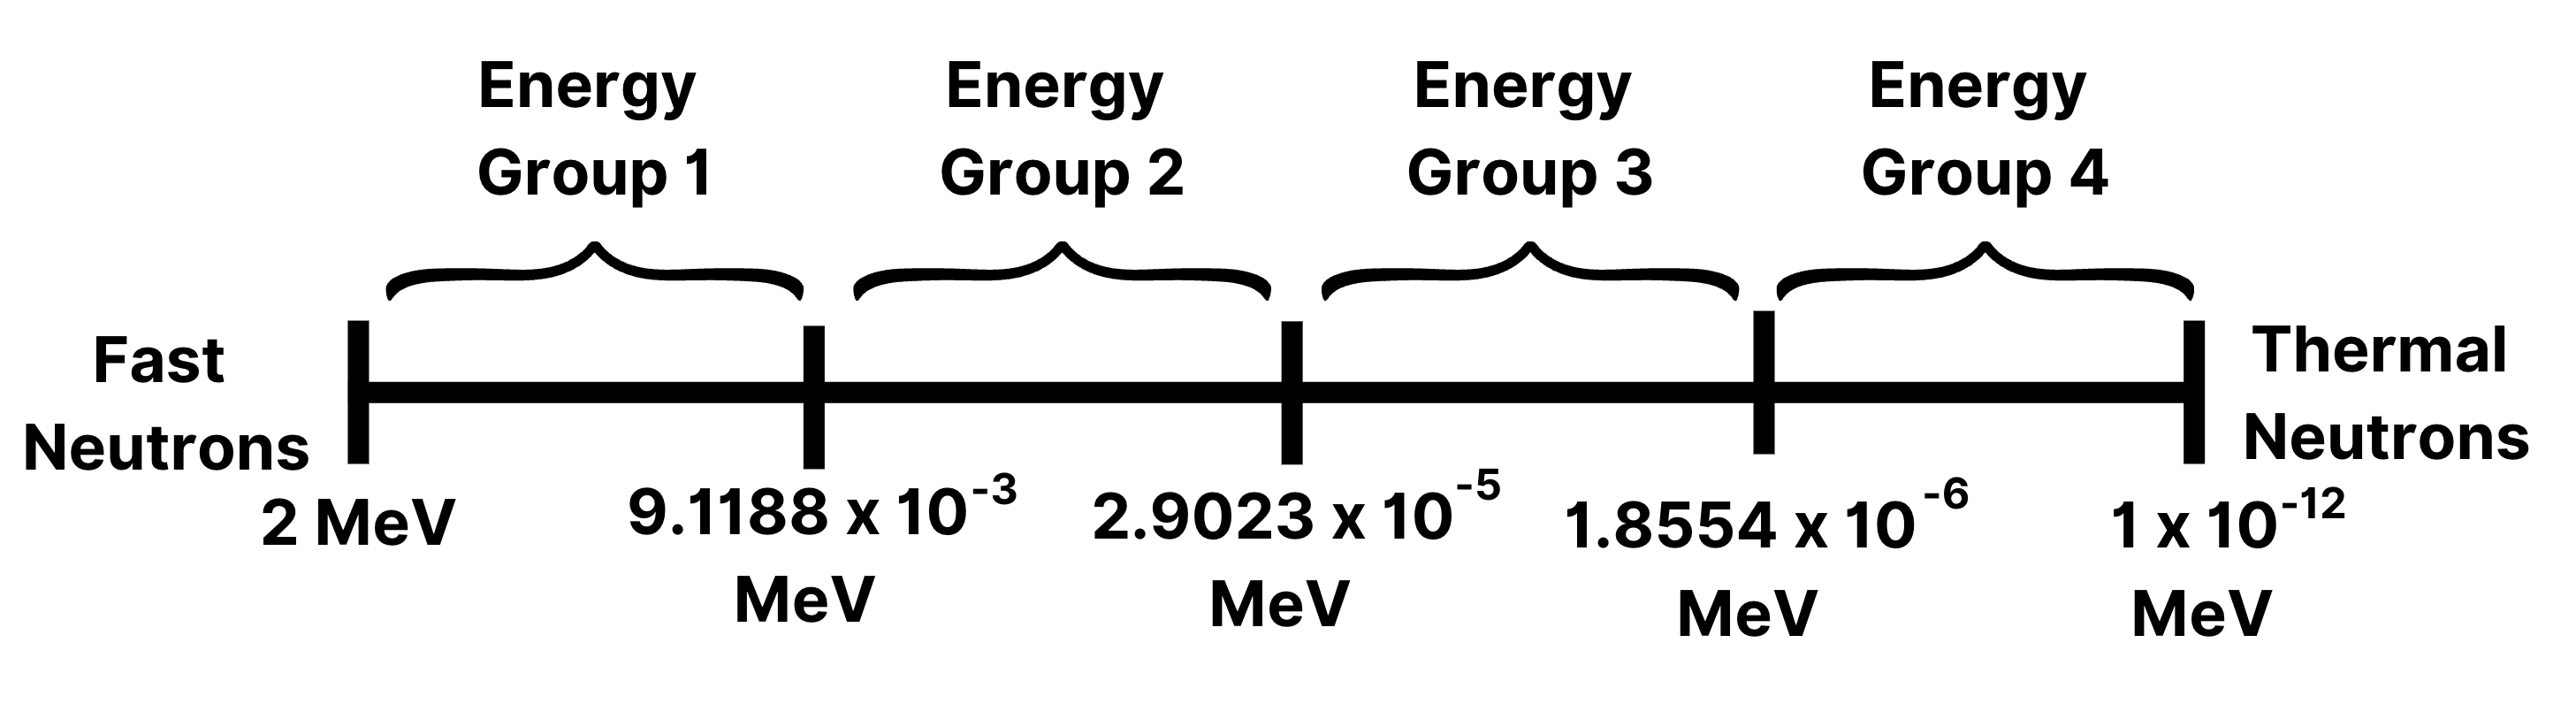
\includegraphics[width=\linewidth]{figures/four-group-structure.png}
        \end{figure}
\end{frame}

\begin{frame}
    \frametitle{AHTR Temperature Model Spatial Homogenization}
        \textbf{Fuel assembly 61 cell discretization}: inter-assembly FLiBe, 
        Y-shaped graphite structure, control rod slot FLiBe, graphite spacers, 
        each diamond shape section's inter-plank FLiBe (3), each graphite plank (18), 
        and each fuel stripe (36)
    \begin{figure}[]
            \centering
            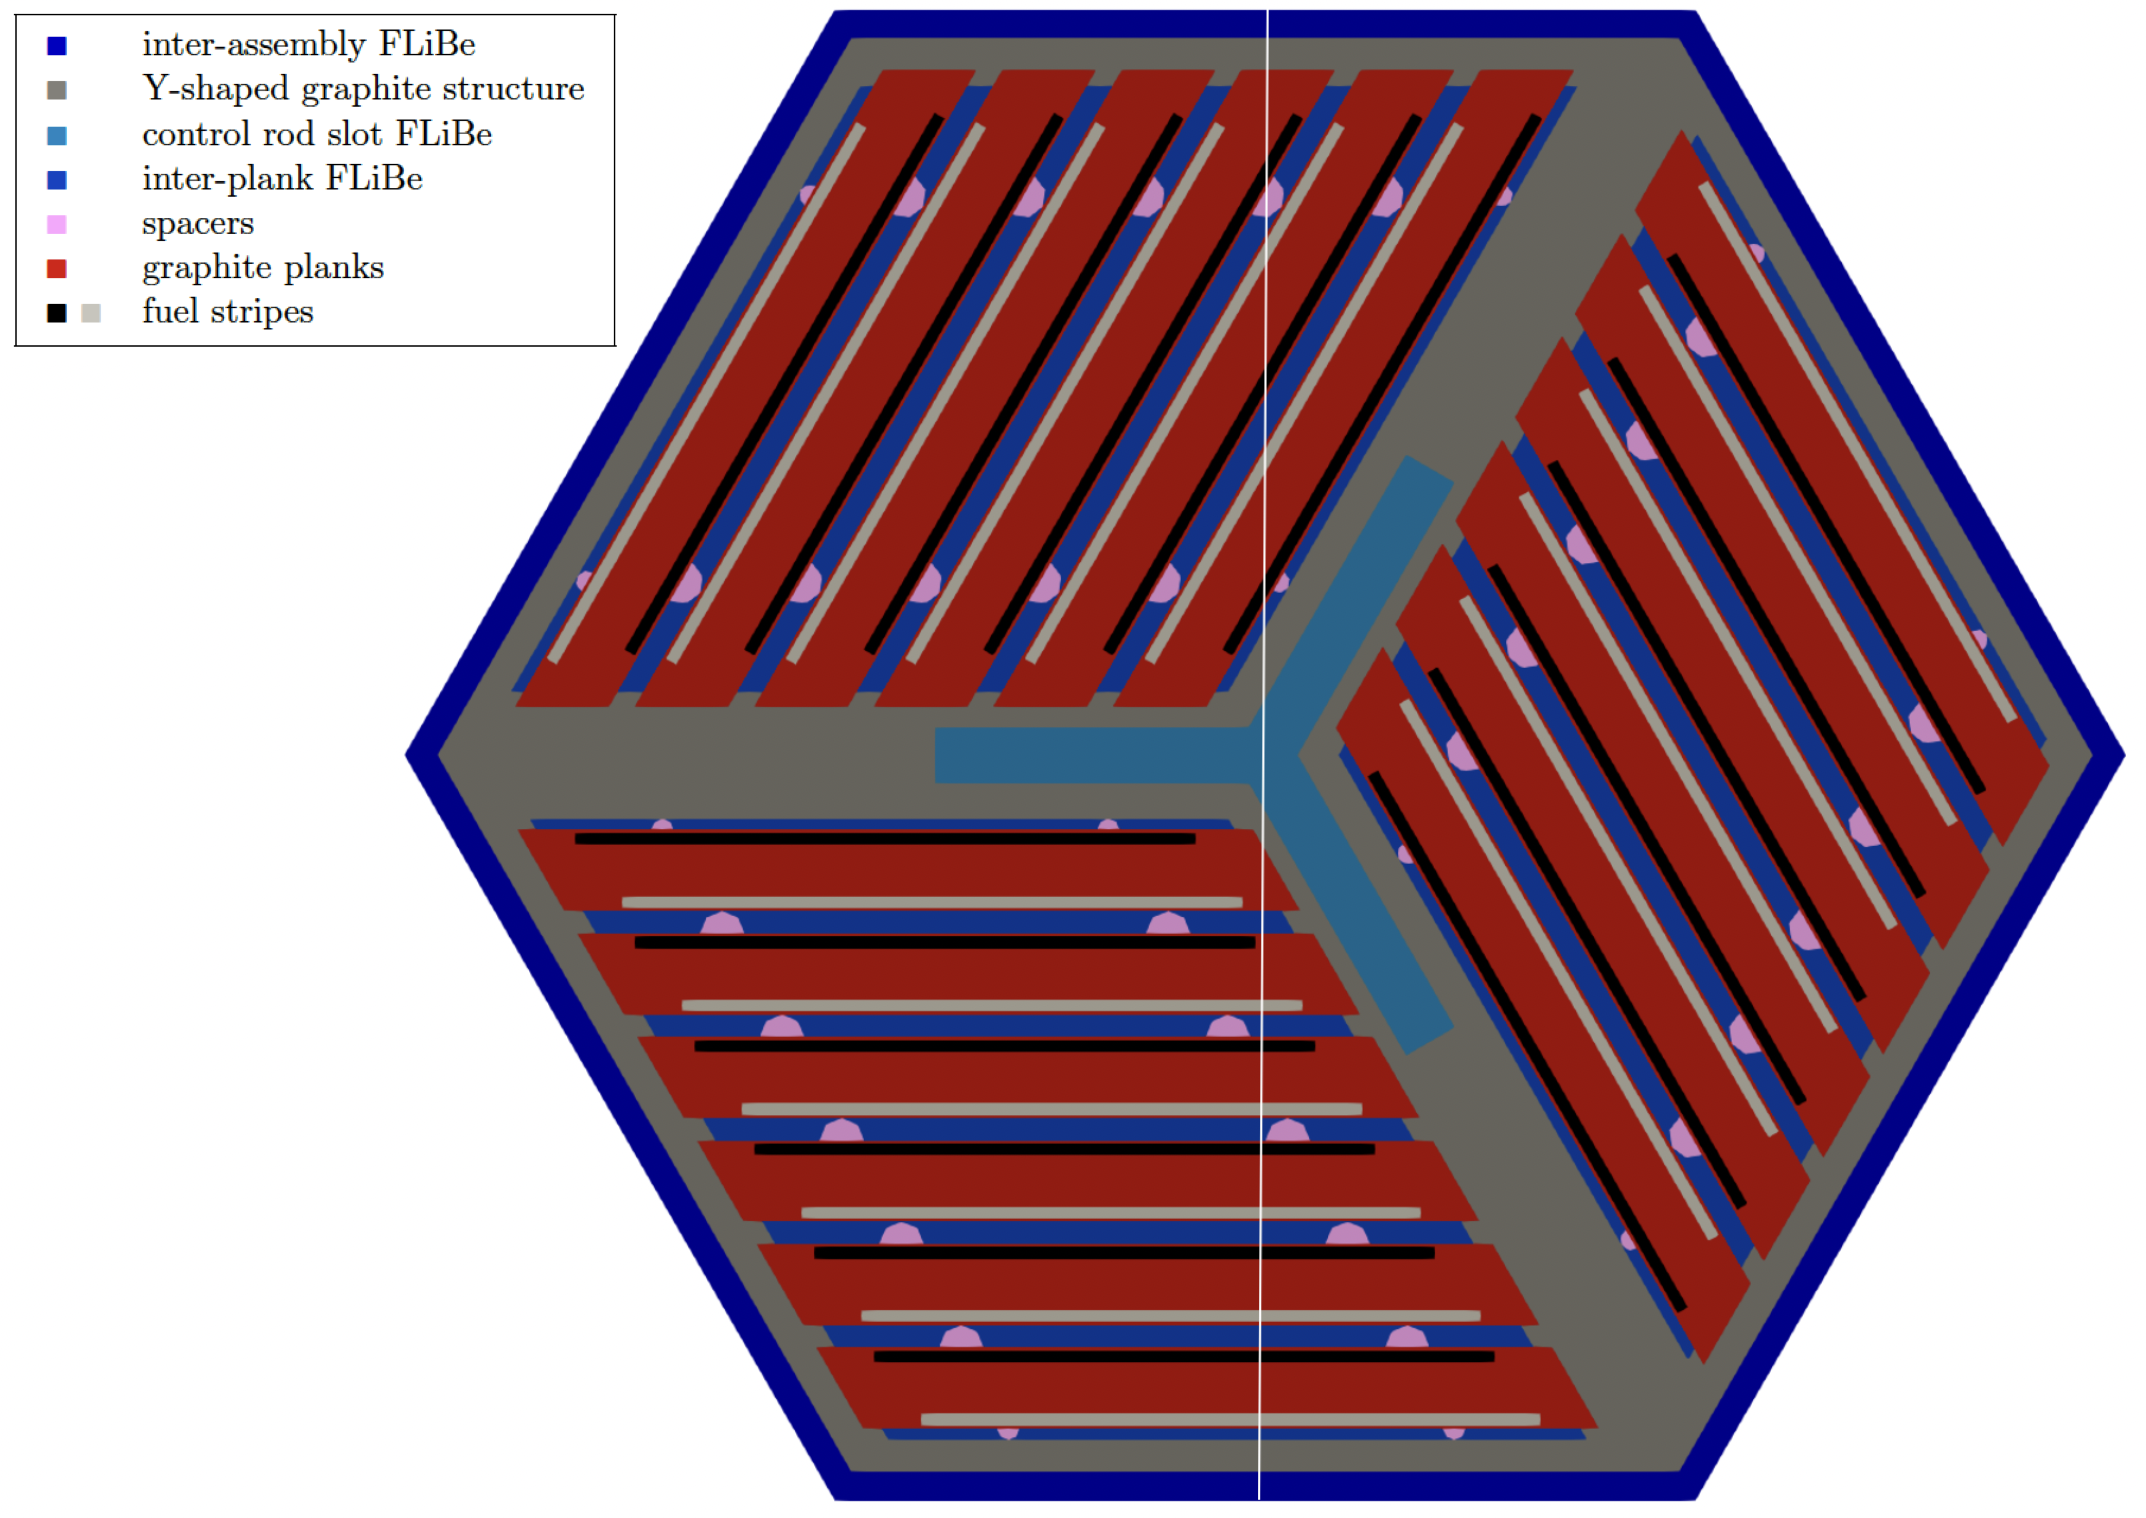
\includegraphics[width=0.9\linewidth]{figures/assembly_mg_pres.png}
        \caption{AHTR assembly spatial homogenization for group constant generation.}
    \end{figure}
\end{frame}

\subsection{Key Neutronics Parameters Verification}
\begin{frame}
    \frametitle{AHTR Temp Model Key Neutronics Parameter Verification}
    \visible<1->{I \textbf{verify acceptable spatial homogenization and energy discretization} by 
    comparing key neutronics parameters (KNPs) between: 
    \begin{itemize} 
        \item OpenMC simulation with continuous energy and TRISO-level spatial fidelity
        \item Moltres simulation with 4-group energy and spatial homogenization
    \end{itemize}}

    \vspace{0.2cm}
    \visible<2->{\textbf{KNPs}: $k_{eff}$, reactivity coefficients, flux distribution, and neutron 
    spectrum
    \begin{itemize}
        \item All comparisons are to verify that the Moltres model is replicating the 
        OpenMC model's neutronics correctly
    \end{itemize}}
    
    \vspace{0.2cm}
    \visible<3->{\textbf{Reactivity coefficients and flux distribution}
    \begin{itemize}
        \item Ensure that \textbf{Moltres accurately calculates the AHTR's temperature 
        distribution}
        \item Reactivity coefficients capture temperature reactivity feedback on the flux
        \item Moltres source term is dependent on flux 
    \end{itemize}}
\end{frame}

\begin{frame}
    \frametitle{Key Neutronics Parameter Verification Summary}
    OpenMC vs Moltres models \textbf{key observations} 
    \begin{itemize}
        \item 216 pcm reactivity difference  
        \item Good agreement in reactivity coefficients and 4-group neutron spectrum
        \item Good agreement in overall flux but larger flux diffs at specific points
    \end{itemize}
    Explanations: 
    \begin{itemize}
        \item Reactivity and flux differences due to Moltres' \textbf{neutron diffusion 
        method} 
        \item Differences in reactivity and flux at specific points might result in 
        \textbf{slightly inaccurate temperatures at certain points}
        \item Since the reactivity coefficients and overall flux distribution 
        are in agreement, this spatial homogenization and energy discretization are 
        \textbf{sufficiently accurate} to calculate and gain an \textbf{overall perspective} 
        of the AHTR's temperature distribution
    \end{itemize}
    Methodology 
    \begin{itemize}
        \item I use this same Moltres model verification method for the AHTR geometries 
        used for optimization 
    \end{itemize}
\end{frame}

\subsection{AHTR Temperature Model Results}
\begin{frame}
    \frametitle{AHTR Temperature Model Results}
    \begin{columns}
        \begin{column}{0.6\textwidth}
            \begin{figure}[]
                \centering
                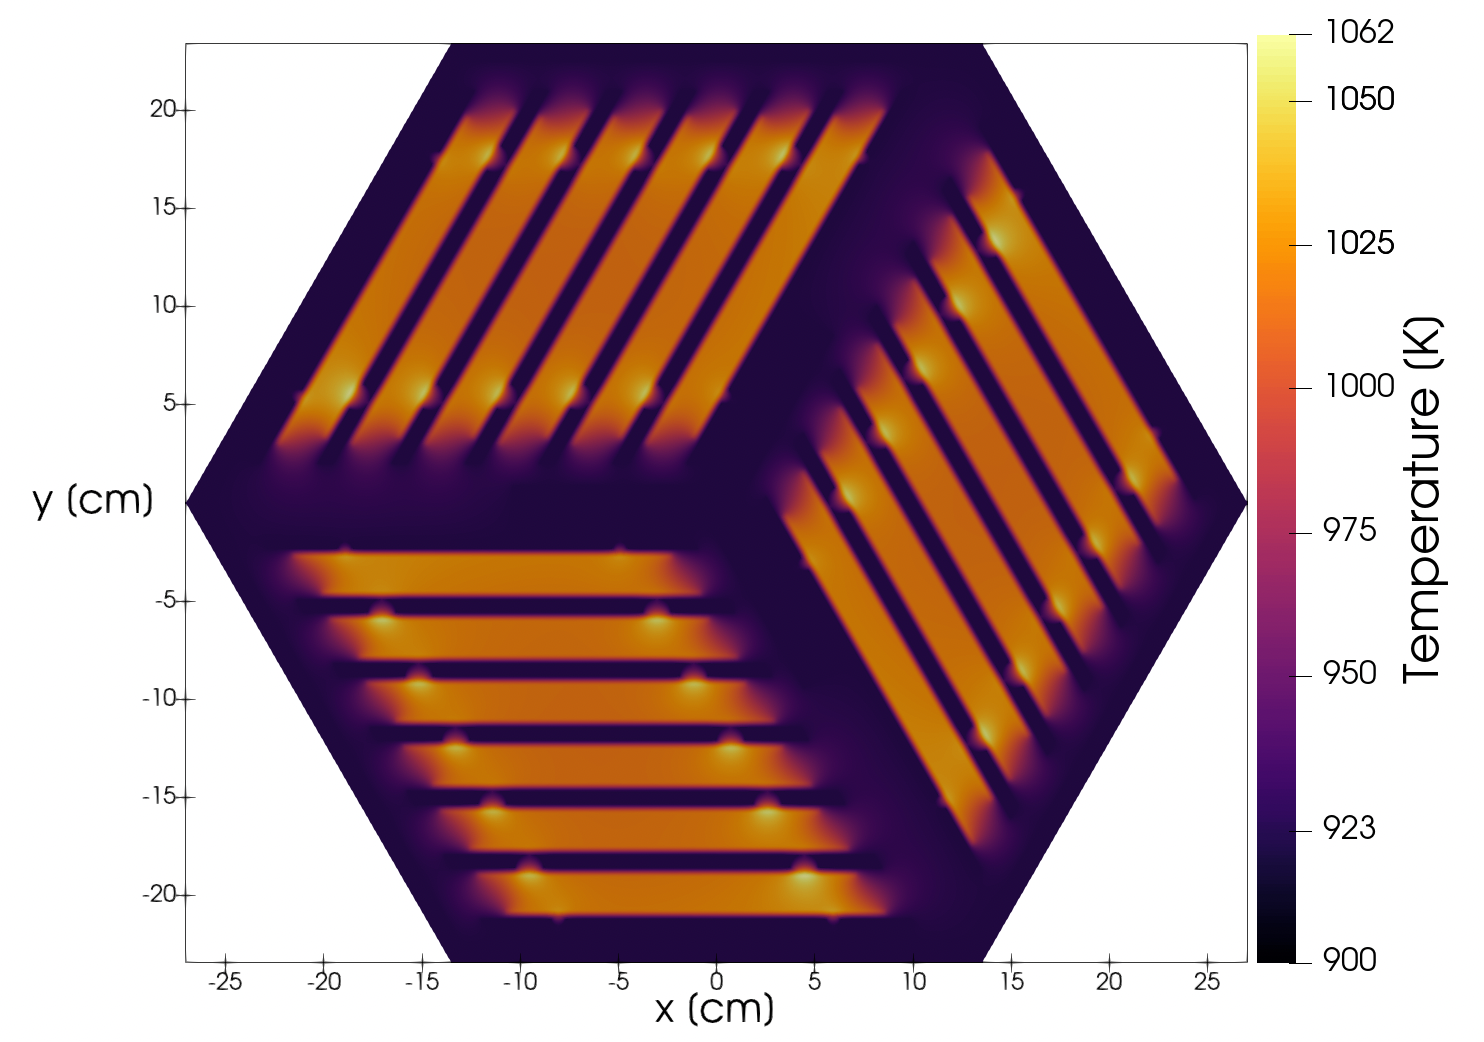
\includegraphics[width=\linewidth]{../docs/figures/benchmark-temperature-model.png} 
                \caption{2D temperature distribution in the \acrfull{AHTR}
                full assembly generated by Moltres.}
            \end{figure}
        \end{column}
        \begin{column}{0.4\textwidth} 
            \begin{block}{Results}
                \begin{itemize}
                    \item Average temperature distribution across the fuel planks are 
                    $\approx 1025K$
                    \item Average temperature of graphite structure is $\approx 935K$
                    \item Temperature peaks at 1062K in the fuel stripes near the spacers
                    \item This is due to the spacers displacing coolant and providing extra 
                    moderation 
                \end{itemize}
            \end{block}
        \end{column}
        \end{columns}
\end{frame}

\subsection{Summary}
\begin{frame}
    \frametitle{FHR Benchmark + AHTR Temperature Model: Summary}
    \begin{block}{I Successfully Completed AHTR Model Development Research Objectives}
        \begin{itemize}
            \item I participated in the OECD-NEA's FHR Benchmark Phases I-A and I-B
            \item I modeled the \gls{AHTR}'s temperature distribution with Moltres
        \end{itemize}
    \end{block}
    \begin{block}{Major Takeaways}
        \begin{itemize}
            \item AHTR has passive safety behavior with negative temperature coeffcients
            \item Increased fuel packing does not always correspond with increased 
            $k_{eff}$ due to self-shielding effects 
            \item These results hint at the possibility of \textbf{minimizing fuel required by 
            optimizing for heterogenous fuel distributions} within the core
            \item AHTR temperature peaks in the fuel stripes near the spacers 
        \end{itemize}
    \end{block}
\end{frame}
